\def\lncs{0}


\ifnum\lncs=0
  \documentclass[11pt]{article}
  \usepackage[top=3cm, bottom=3cm, left=2cm, right=2cm]{geometry}      % [top=2cm, bottom=2cm, left=2cm, right=2cm]
  \geometry{letterpaper}                   % ... or a4paper or a5paper or ...
  %\geometry{landscape}                % Activate for for rotated page geometry
  %\usepackage[parfill]{parskip}
  \usepackage{amsthm}
  \newtheorem{theorem}{Theorem}
  \newtheorem{lemma}[theorem]{Lemma}
  \newtheorem{proposition}[theorem]{Proposition}
  \newtheorem{corollary}[theorem]{Corollary}
  \newtheorem{conjecture}{Conjecture}
  \newtheorem{definition}{Definition}
  \newtheorem{assumption}{Assumption}
  \newtheorem{claim}{Claim}
  \newtheorem{problem}{Problem}
  \newtheorem{construction}{Construction}
  \newtheorem{remark}{Remark}
  \renewcommand{\vec}[1]{\vect{#1}}      % activate for lncs style vectors

\else
  \documentclass{llncs}
  \newtheorem{construction}{Construction}
  \renewcommand{\paragraph}[1]{\subsubsection{#1}}
\fi

\usepackage[dvipsnames]{xcolor}

\usepackage{tikz}
\usepackage{graphicx}
\usepackage{csquotes}
\usepackage{multirow}
\usepackage{amssymb, amsmath, amsfonts}
\usepackage{enumerate}
\usepackage{hyperref}
\usepackage{xspace}
\usepackage{graphicx}
\usepackage{latexsym}
\usepackage{color}
\usepackage{framed}
\usepackage{algpseudocode}
\usepackage{breakcites}

\mathchardef\mhyphen="2D
\newcommand{\secref}[1]{\mbox{Section~\ref{#1}}}
\newcommand{\subsecref}[1]{\mbox{Subsection~\ref{#1}}}
\newcommand{\apref}[1]{\mbox{Appendix~\ref{#1}}}
\newcommand{\thref}[1]{\mbox{Theorem~\ref{#1}}}
\newcommand{\exref}[1]{\mbox{Example~\ref{#1}}}
\newcommand{\defref}[1]{\mbox{Definition~\ref{#1}}}
\newcommand{\corref}[1]{\mbox{Corollary~\ref{#1}}}
\newcommand{\lemref}[1]{\mbox{Lemma~\ref{#1}}}
\newcommand{\assref}[1]{\mbox{Assumption~\ref{#1}}}
\newcommand{\probref}[1]{\mbox{Problem~\ref{#1}}}
\newcommand{\clref}[1]{\mbox{Claim~\ref{#1}}}
\newcommand{\propref}[1]{\mbox{Proposition~\ref{#1}}}
\newcommand{\remref}[1]{\mbox{Remark~\ref{#1}}}
\newcommand{\consref}[1]{\mbox{Construction~\ref{#1}}}
\newcommand{\figref}[1]{\mbox{Figure~\ref{#1}}}
\newcommand{\conditionalpara}[1]{
\ifnum\lncs=1\noindent \textbf{#1} \else \paragraph{#1}\fi}
\newcommand{\conditionaleqn}[1]{\ifnum\lncs=1$#1$\else \[#1\]\fi}
\DeclareMathOperator*{\expe}{\mathbb{E}}
\DeclareMathOperator*{\var}{\text{Var}}
\DeclareMathOperator*{\Exp}{\mathbb{E}}
\DeclareMathOperator*{\argmax}{arg\,max}
\DeclareMathOperator*{\argmin}{arg\,min}

% Commands
\newcommand{\comment}[1]{\textcolor{Mulberry}{#1}}
\newcommand{\todo}[1]{\textcolor{red}{TODO: #1}}
%\newcommand{\todo}[1]{}
\newcommand{\here}{\todo{Stopped here! }}

%Probability
\newcommand{\Ex}[1]{\Exp\left[#1\right]}
\newcommand{\Exlim}[2]{\Exp\limits_{#1}\br{#2}}
\newcommand{\Prob}[1]{\Pr\br{#1}}
\newcommand{\Problim}[2]{\Pr\limits_{#1}\br{#2}}
\newcommand{\p}[1]{p\prns{#1}}

% Entropy
\newcommand{\ent}[1]{\mathrm{H}\prns{#1}}
\newcommand{\minent}[1]{\mathrm{H}_{\infty}\prns{#1}}
\newcommand{\acminent}[2]{\tilde{\mathrm{H}}_{\infty}\prns{#1|#2}}
\newcommand{\acminenteps}[2]{\tilde{\mathrm{H}}_{\infty}^\epsilon\prns{#1|#2}}
\newcommand{\hart}[1]{\mathrm{H}_0\prns{#1}}


%MACROS galore!!!
\newcommand{\class}[1]{{\ensuremath{\mathsf{#1}}}}
\newcommand{\gen}{\ensuremath{\class{Gen}}\xspace}
\newcommand{\aux}{\ensuremath{\class{Advice}}\xspace}
\newcommand{\advice}{\ensuremath{\class{advice}}\xspace}
\newcommand{\rep}{\ensuremath{\class{Rep}}\xspace}
\newcommand{\sketch}{\ensuremath{\class{SS}}\xspace}
\newcommand{\viable}{\ensuremath{\mathtt{Viable}}\xspace}
\newcommand{\rec}{\ensuremath{\class{Rec}}\xspace}
\newcommand{\enc}{\ensuremath{\class{Enc}}\xspace}
\newcommand{\wt}{\ensuremath{\textsf{wt}}\xspace}
\newcommand{\dec}{\ensuremath{\class{Dec}}\xspace}
\newcommand{\prg}{\ensuremath{\class{prg}}\xspace}
\newcommand{\zo}{\ensuremath{\{0, 1\}}}
\newcommand{\vect}[1]{\ensuremath{\mathbf{#1}}}
\newcommand{\zq}{\ensuremath{\mathbb{Z}_q}}
\newcommand{\Fq}{\ensuremath{\mathbb{F}_q}}
\newcommand{\sample}{\ensuremath{\class{Sample}}\xspace}
\newcommand{\neigh}{\ensuremath{\class{Neigh}}\xspace}
\newcommand{\error}{\ensuremath{\class{Err}}\xspace}
\newcommand{\weight}{\ensuremath{\class{Wgt}}\xspace}
\newcommand{\dis}{\ensuremath{\mathsf{dis}}}
\newcommand{\bin}{\ensuremath{\mathsf{Bin}}}
\newcommand{\decode}{\ensuremath{\mathsf{Decode}}}
\newcommand{\guess}{\mathsf{guess}}
\newcommand{\nullsp}{\mathtt{null}}


\newcommand{\A}{\mathcal{A}}
\newcommand{\F}{\mathbb{F}}


\newcommand{\metric}{\ensuremath{\mathtt{Metric}}\xspace}
\newcommand{\bdde}{\ensuremath{\mathtt{BDDE}}\xspace}
\newcommand{\bdders}{\ensuremath{\mathtt{BDDE-RS}}\xspace}
\newcommand{\bdderl}{\ensuremath{\mathtt{BDDE-RL}}\xspace}
\newcommand{\findrep}{\ensuremath{\mathtt{FIND-REP}}\xspace}
\newcommand{\hill}{\ensuremath{\mathtt{HILL}}\xspace}
\newcommand{\hillrlx}{\ensuremath{\mathtt{HILL\mhyphen rlx}}\xspace}
\newcommand{\yao}{\ensuremath{\mathtt{Yao}}\xspace}
\newcommand{\unp}{\ensuremath{\mathtt{unp}}\xspace}
\newcommand{\unprlx}{\ensuremath{\mathtt{unp\mhyphen rlx}}\xspace}
\newcommand{\metricstar}{\ensuremath{\mathtt{Metric}^*}\xspace}
\newcommand{\metricd}{\ensuremath{\mathtt{Metric}^*\mathtt{-d}}\xspace}
\newcommand{\hillstar}{\ensuremath{\mathtt{HILL}^*}\xspace}
\newcommand{\hillprime}{\ensuremath{\mathtt{HILL'}}\xspace}
\newcommand{\metricprime}{\ensuremath{\mathtt{Metric'}}\xspace}
\newcommand{\metricprimestar}{\ensuremath{\mathtt{Metric'}^*}\xspace}
\newcommand{\hillprimestar}{\ensuremath{\mathtt{HILL'}^*}\xspace}
\newcommand{\poly}{\ensuremath{\mathtt{poly}}\xspace}
\newcommand{\rank}{\ensuremath{\mathtt{rank}}\xspace}
\newcommand{\ngl}{\ensuremath{\mathtt{ngl}}\xspace}
\newcommand{\Hoo}{\mathrm{H}_\infty}
\newcommand{\Hav}{\tilde{\mathrm{H}}_\infty}
\newcommand{\Haveps}{\tilde{\mathrm{H}}_\infty^\epsilon}
\newcommand{\goodsketch}{\ensuremath{\mathsf{GoodSketch}}\xspace}
\newcommand{\goodkey}{\ensuremath{\mathsf{GoodKey}}\xspace}
\newcommand{\Hfuzz}{\mathrm{H}^{\mathtt{fuzz}}_{t,\infty}}
\newcommand{\Wallfuzz}{\mathcal{W}_{\mathtt{fuzz}}^{\mathtt{all}}}
\newcommand{\Huse}{\mathrm{H}_{\mathtt{usable}}}
\newcommand{\Dom}{\mathsl{Dom}}
\newcommand{\Range}{\mathsl{Rng}}
\newcommand{\Keys}{\mathsl{Keys}}
\def\col{\mathrm{Col}}




% Useful Notation
\newcommand{\defined}{:=}
\newcommand{\sbr}[1]{ \!\left\{ #1 \right\} }
\newcommand{\br}[1]{\!\left[#1\right]}
\newcommand{\prns}[1]{\!\left(#1\right)}
\renewcommand{\log}[1]{\mathsf{log}\prns{#1}}
\newcommand{\zeroone}[1]{\sbr{0,1}^{#1}}

\newcommand{\anote}[1]{\textcolor{blue}{[ACR: #1]}}

\title{Impossibility of Efficient Information-Theoretic Fuzzy Extraction}
\ifnum\lncs=0
\author{Luke Demarest\\University of Connecticut\\luke.h.demarest@gmail.com \and Benjamin Fuller\\University of Connecticut\\benjamin.fuller@uconn.edu\and Alexander Russell\\University of Connecticut\\acr@uconn.edu}
\fi
\date{\today}

% Document
\begin{document}
  
  \maketitle
  %!TEX root = main.tex

\abstract{
Fuzzy extractors convert noisy signals from the physical world into reliable cryptographic keys.  %An important open question is building fuzzy extractors that secure all possible distributions.  
Fuzzy min-entropy upper bounds the length of the key that can be derived from a distribution (Fuller, Reyzin, and Smith, IEEE Transactions on Information Theory 2020).  Specifically, fuzzy min-entropy is proportional to the sum of the probability of nearby points, such points are transformed to the correct key and suffice for adversary success. Fuzzy min-entropy that is superlogarithmic in the security parameter is required for a noisy distribution to be suitable for key derivation.
 
There is a wide gap between what is possible with respect to computational and information-theoretic adversaries.  A good obfuscator derives keys from all distributions with superlogarithmic entropy.

Against information-theoretic adversaries, it is impossible to build a single fuzzy extractor that works for all distributions (Fuller, Reyzin, and Smith, IEEE Transactions on Information Theory 2020). A weaker goal is to build a fuzzy extractor for each probability distribution.  This is the approach taken by Woodage et al. (Crypto 2017).  Prior approaches use the full description of the probability mass function and are inefficient.
We show this is inherent: \textbf{for most distributions with $2^k$ points there is no secure fuzzy extractor that uses less  $\Theta(k2^k)$ bits of information about the distribution.}  This result rules out the possibility of efficient, information-theoretic fuzzy extractors for most distributions with fuzzy min-entropy.

We show an analogous result with stronger parameters for information-theoretic secure sketches. Secure sketches are frequently used to construct fuzzy extractors. 
}
  \pagebreak
  %!TEX root = main.tex

% Introduction for negFE
\section{Introduction}
Infromation reconciliation and privacy amplification are the two fundamental tasks for key derivation from noisy sources.  Applications areas include quantum key agreement, biometrics, and physically uncloneable functions~\cite{bennett1988privacy,dodis2008fuzzy}. Secure sketches perform information reconciliation non-interactively.  They consist of a pair of algorithms sketch or $\sketch$ where $\sketch(w) = ss$ should reveal as little information as possible about $w$ while still allowing one to reconstruct $w$ from a nearby $w'$. That is, it should be the case that for all nearby $w', \rec(w', ss) = w$.  These two properties are in tension because allowing recovery of $w$ requires information about $w$.  Upper bounds on the unpredictability of $w | ss$ are related to the size of the best error-correcting codes~\cite{dodis2008fuzzy,fuller2020computational}. 

  Fuzzy extractors additionally perform privacy amplification, converting $w$ into a uniform value.  They consist of a pair $(\gen, \rep$) where $(r, p)\leftarrow \gen(w)$ is indistinguishable from $(u, p)$ and $\rep(w', p) =r$.

Throughout the Introduction, we use the notation of fuzzy extractors and note when there are material differences for secure sketches.
Since noisy sources come from the physical world the goal is to be able to support as many distributions $W$ as possible.  Fuller, Reyzin, and Smith~\cite{fuller2016fuzzy,fuller2020fuzzy} identified the notion of fuzzy min-entropy $\Hfuzz(W)$ which measures the adversary's success when given oracle access to $\rep(\cdot, p)$ but is unable to learn anything from the value  $p$.  Mathematically, for a distance $t$, specifying which points are nearby, fuzzy min-entropy quantifies the weight of the heaviest ball in the probability mass function of $W$.  That is, 
\[
\Hfuzz(W):= -\log{\max_{w'} \sum_{w | \dis(w, w')\le t} \Pr[W=w]}.
\]A primary goal of fuzzy extractors is to build a single fuzzy extractor that works for the family of all distributions $\Wallfuzz = \{ W | \Hfuzz(W) = \omega(\log \lambda)\}$ for some security parameter $\lambda$.  We call such a fuzzy extractor \emph{universal} as it simultaneously works for any secureable distribution $W$. 
If one desires computational security, a universal fuzzy extractor is achievable using general obfuscation~\cite{BarakBCKPS13,BitanskyCKP14,bitansky2017virtual} or specific number-theoretic assumptions~\cite{galbraith2019obfuscated}. 


The situation for information-theoretic security is more complicated.\footnote{Fuzzy extractors were first designed as an information-theoretic primitive because of strong connections to randomness extraction and coding theory.  Many constructions consist of an information-theoretic secure sketch and a (computational) randomness extractor.  The secure sketch is analyzed using information-theoretic techniques.  Computational tools are used primarily to amplify privacy~\cite{wen2018robustly,wen2019generic}.  (Exceptions exist such as the universal constructions listed above and constructions for distributions with additional properties~\cite{apon2017efficient,alamelou2018pseudoentropic,fuller2020computational,canetti2021reusable}.)
}  Fuller, Reyzin, and Smith~\cite{fuller2020fuzzy} showed that it is impossible to build a universal fuzzy extractor with information-theoretic security.  More precisely, they constructed a family of distributions $\mathcal{W}'$ and showed that any fuzzy extractor $(\gen, \rep)$ must be insecure for an average member of $\mathcal{W}'$. We use the notation $W_Z$ to indicate uniform sampling from the family $\mathcal{W}'$ with $Z$ describing the chosen distribution.  Importantly, in the impossibility result, the adversary knows the entire description of the chosen distribution $Z$ but not the individual point $w$ that was input to $\gen$.

On the positive side, multiple works~\cite{hayashi2014secret,hayashi2016secret,fuller2016fuzzy,woodage2017new,tyagi2017universal,TVW18,LA18,fuller2019continuous,fuller2020fuzzy} presented a construction that works for each $W_Z\in \Wallfuzz$.  This is called the \emph{distribution-sensitive} setting as $\gen$ also knows the entire probability mass function $Z$ of the chosen $W_Z$, denoted as $\gen_{W_Z}, \rec_{W_Z}$.  All constructions in this line are computationally inefficient; for an input point $w$ they look up the probability that $\Pr[W_Z=w]$ and the probability of points $w'$ where $\dis(w, w')\le t$.  
%Thus, there is a large gap between the state of affairs with computational and information-theoretic security.  With computational security, universal fuzzy extractors are possible.  With information-theoretic security universal fuzzy extractors are impossible.  Furthermore, known distribution-sensitive fuzzy extractors require information about $W$ proportional to its description.  
We show this inefficiency is inherent:

\begin{displayquote}
\textbf{Any distribution-sensitive information-theoretic fuzzy extractor requires an exponential amount of information about the distribution $W$.  For most distributions $W \in \Wallfuzz$, a distribution-sensitive fuzzy extractor cannot be efficiently implemented.} 
\end{displayquote} 
Our results are for the Hamming metric over $\zo^n$. We show that for most distributions $W$ where $\Hfuzz(W) := \gamma$ building a good fuzzy extractor requires having approximately $\gamma 2^\gamma$ bits of information about the distribution.\footnote{To be more precise,  we consider distributions that have $2^k$ points where $k = \gamma + c n$ for an arbitrary constant $c>0$.}
The relevant parameter regimes of impossibility are shown in Figure~\ref{fig:param regime}.  The two most important parameters are the noise rate $t/n$ and the fuzzy entropy rate $\gamma/n$. The area under the curves represents parameters where the construction is impossible for an average distribution with those parameters unless one has an exponential amount of information about the distribution.  All results hold for a constant fraction of the distributions with the presented parameters.

In spirit, our result rules out constructions that do not have a full description of the probability mass function written in their description.  Our results do not restrict the running time or size of the fuzzy extractor algorithms, only how much information is known about the distribution $W$ being secured.  





There are (at least) two natural interpretations of the above result: 1) that fuzzy min-entropy does not measure the suitability of distributions for key derivation or 2) that efficient fuzzy extractors are an inherently computational object.

\paragraph{The notion of fuzzy min-entropy}
One of the principal components of a fuzzy extractor is privacy amplification where smooth conditional min-entropy is a necessary and sufficient condition.  This places efficient privacy amplification as an information-theoretic object.  However, the gap between necessary and sufficient conditions for efficient primitives that perform information reconciliation appears much wider. The only known \emph{efficient} constructions for information reconciliation fall into one of two categories:
\begin{description}
\item[High entropy] If the source $W$ has high entropy $\Hoo(W)\ge \omega(\log n) + \log{|B_t|}|$ (where $|B_t|$ is the size of a Hamming ball of radius $t$) then one can build a good secure sketch by writing down the syndrome of an error correcting code which corrects $t$ errors.  This syndrome construction  leaks at least $\log{|B_t|}$ bits of information about $W$.\footnote{A construction that leaks only $\log{|B_t|}$ bits about $W$ requires a perfect code which are rarely achievable.}  Unfortunately, this construction provides no guarantee when $\Hoo(W)< \log{|B_t|}$ which is the case for biometrics, see \cite[Proposition 1]{canetti2021reusable} and \cite[Introduction]{simhadri2019cryptographic}.
\item[Highly structured] Sources where each bit is i.i.d.\,can be analyzed using Shannon entropy.  In this setting, key rate asymptotically approaches $\Hfuzz(W)$ if one assumes the second reading $w'$ will be uniformly distributed in the ball around the first reading~\cite[Theorem 2]{tuyls2004capacity}.  Unfortunately, dimensions of real-physical sources are rarely i.i.d.~\cite{daugman2004}.
\end{description}

There isn't an obvious sufficient condition to use instead of fuzzy min-entropy.  Various weaker structured conditions have been used in the computational regime but with little evidence that physical sources have these properties~\cite[Figure 1]{demarest2021code} and \cite{simhadri2019cryptographic}. A desirable research direction is to find statistical properties found by physical sources that bypass our negative results. 

\paragraph{Fuzzy extractors are computational objects} The other natural explanation of the result is that non-interactive information-reconciliation should be considered a computational object. This is our preferred interpretation since one can build universal (and efficient) fuzzy extractors if computational security suffices.  We note that the only known constructions assume either general obfuscation~\cite{BarakBCKPS13,BitanskyCKP14,bitansky2017virtual} or specific number-theoretic assumptions that are not well studied~\cite{galbraith2019obfuscated}. Thus, an important piece of research is to understand the required assumptions to build efficient, universal fuzzy extractors with computational security. 

\begin{figure}[t]
\centering
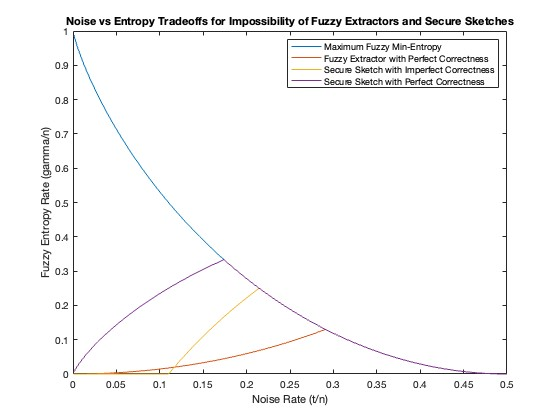
\includegraphics[width=.9\textwidth]{EntropyvsError.jpg}
\caption{The region of error rate $t/n$ ($x$-axis) and fuzzy entropy rate $\gamma/n$ (y-axis) pairs for which the two negative results apply.  The six curves are maximum fuzzy min-entropy $\gamma/n = (1-h_2(t/n))$, Theorem~\ref{thm:main theorem}, Theorem~\ref{thm:main theorem ss} with $\delta=.25$,  Theorem~\ref{thm:main theorem ss} with $\delta =0$, \cite[Theorem 5.1]{fuller2020fuzzy} and \cite[Theorem 7.2]{fuller2020fuzzy}. The parameter $\delta$ is how frequently the secure sketch is allowed to be incorrect.  We consider fuzzy extractors with perfect correctness where $\delta=0$.}
\label{fig:param regime}
\end{figure}

\subsection{Proof Techniques}
Our results are information-theoretic in nature. Recall that we consider a family of distributions $\mathcal{W}$ and use $W_Z$ to denote sampling a random distribution from $\mathcal{W}$ with $Z$ describing the distribution.  Lastly, we use $w\leftarrow W_Z$ to denote sampling a point from the distribution.  We show the impossibility of two types of fuzzy extractors:
\begin{description}
\item[Def.~\ref{def:fe distributional}] (Universal) Fuzzy extractors with distributional advice.  This is triple of algorithms $(\advise, \gen, \rep)$ designed to work for all $W_Z \in \mathcal{W}$ where $\mathcal{W}$ consists of all distributions with a certain amount of fuzzy min-entropy for a fixed error tolerance $t$.  However, the fuzzy extractor is given information about $Z$.  Namely, there is a deterministic algorithm $\advise = \advise(Z)$. Then both $\gen$ and $\rep$ are given $\advise$. $\gen(w, \advise)$ has to produce a uniform key.  All information about $Z$ given to $\gen$ is contained in $\advise$ and the point $w$.
\item[Def.~\ref{def:fe}] Space bounded fuzzy extractors for a specific distribution $W$ are required to have a bounded size description of $(\gen, \rep)$.
\end{description}

We show impossibility of building a fuzzy extractor with distributional advice of length $\ell$ for $\mathcal{W}$ implies impossibility of building a space bounded fuzzy extractor for length $\ell$ (Lemma~\ref{lem:distributional advise suffices}). 
The core of our negative results is to show impossibility of building fuzzy extractors with distributional advice.   Before introducing our proof techniques we perform a brief overview of Fuller, Reyzin, and Smith's~\cite{fuller2020fuzzy} impossibility result.

\paragraph{Review of Fuller, Reyzin, and Smith~\cite{fuller2020fuzzy}}
The correctness constraint of a fuzzy extractor says that for $(r, p)\leftarrow \gen(w)$ for all $w'$ close to $w$ the correct key is reproduced, i.e. $\rep(w', p)=r$.  As such, one can partition the input space $\zo^n$ by what value of $r$ the point  $v\in \zo^n$ produces.  Values $v$ that could have produced  $r$ will be at least distance $t$ from the boundary of this partition, we call the set of such $v$, $\viable_{r,p}$.  $\viable_{r,p}$ can be bounded geometrically using the isoperimetric inequality~\cite{harper1966optimal}.  This bound applies for any distribution over the inputs $w$.

Consider the following simple distinguisher for a triple $r, p, z$.  One computes the key partition described above and the set $\viable_{r,p}$. If $\viable_{r,p} \cap W_Z =\emptyset$ output the key is random, otherwise output key is real.
The core of Fuller, Reyzin, and Smith's impossibility was to build a family $\mathcal{W}^{FRS}$ with three properties:
\begin{enumerate}
\item The distribution was $2$-universal~\cite{carter1977universal}, so the remainder of the distribution was unknown conditioned on the input $w$. 
\item Distributions $W_Z \in \mathcal{W}^{FRS}$ shared few points, and 
\item Each distribution $\mathcal{W}^{FRS}$ had fuzzy min-entropy.
\end{enumerate}
Together these three properties meant that for any partition most distributions $W_Z$ would have few nonempty interiors and the real key could be distinguished from a uniform key.  
The family is as follows: let $\mathbf{C}$ be a linear error-correcting code with distance $t$, let $\mathbf{H}$ be its syndrome, let $c$ be a coset.  Then each $Z = (\mathbf{H}, c)$ is the set of all points $\{w | \mathbf{H} w = c\}$.

\paragraph{Moving to the distributional advice setting}
To set notation for the distributional advise game, we consider the following game for a tuple of algorithms $(\advise, \gen, \rep)$:
\begin{enumerate}
\itemsep0em
\item A uniform sample from $W_z\leftarrow \mathcal{W}$ where $z$ describes the distribution.
\item A bounded length $\advise = \advise(z)$ is computed.
\item One computes $w\leftarrow W_z$.
\item The algorithm computes $(r, p)\leftarrow \gen(w, \advise)$.
\item The adversary is given either $(r, p, z)$ or $(u, p, z)$ for a uniform $u$.
\end{enumerate}

In \cite{fuller2020fuzzy}, the only information that $\gen$ had about $z$ was the input point $w$.  In our setting, $\gen$ gets $\advise$.  Fuller, Reyzin, and Smith's family had a short description so $\advise$ could completely write $Z$, allowing $\gen$ to align the interior of the parts with points in $W_Z$.  Thus, it is clear that the distributional advise setting requires a distribution with no short description.  It also requires showing that aligning the interior of the parts is difficult given an arbitrary bounded length advise.  Both problems can be approached by removing the structure from the family and considering the set of all distributions $W_Z\in\mathcal{W}$ with fuzzy min-entropy at least $\gamma$. 

This distribution is statistically close to the set of all distributions with $2^k$ points chosen uniformly without replacement where $k = \gamma +cn$ for an arbitrary constant $c>0$.  We call this set of distributions $U_{n,k}$ and let $w_1,...., w_{2^k}$ be the points with nonzero probability.  The key to the proof is showing that as long as $|\advise|$ is shorter than $k2^k$, most points $w_i | \advise$ are unpredictable.  This argument must account for the fact that $\advise$ can choose to completely determine some points or provide equal information about all points. 

The techniques for the secure sketch setting are similar, however, there are stronger geometric bounds on the number of viable points because secure sketches imply Shannon error correcting codes.  Our result considers a secure sketch that retains smooth min-entropy instead of min-entropy.  This is so we can use $U_{n,k}$ throughout the proof and show this implies the hardness of building a secure sketch for all distributions with sufficient fuzzy min-entropy.  

Importantly, both results operate generically in the size of the maximum number of viable points for the relevant primitive.  Such bounds have been well established in the literature due to their connections with coding theory.  This means if one can provide a new bound on fuzzy extractor or secure sketch quality this can be directly used in our results.


\paragraph{Comparing with Fuller, Reyzin, and Smith~\cite{fuller2020computational}}
Our fuzzy extractor result requires the $|r| = \omega(\log n)$.  This is in contrast to Fuller, Reyzin, and Smith~\cite{fuller2020computational} who showed an impossibility for a key length of $3$.\footnote{Similarly, our result for secure sketches requires them to retain at least $\omega(\log n)$ bits of min-entropy about the input in comparison with \cite{fuller2020computational} which required the sketch to maintain $3$ bits of entropy.} This change comes because $\advise$ can supply a lot of information about a small number of points in $W_Z$, allowing $\gen$ to ensure that some $\viable_{r,p}$ are nonempty. Furthermore, all bounds are weaker than those of Fuller, Reyzin, and Smith.  The core of the difference is that since $\mathcal{W}^{FRS}$ the adversary received entirely new information by the leftover hash lemma~\cite{haastad1993construction,barak2011leftover}. In our setting, we argue about the expected number of points in $W_Z$ that are included in the $\viable$ region. 

Our secure sketch result also considers an object that retains smooth conditional min-entropy~\cite{renner2005simple} which is a weaker object than traditional min-entropy.  This is so we can conduct the argument using $U_{n,k}$ and ``smooth'' to a family with fuzzy min-entropy. Smooth conditional min-entropy is the necessary condition for conversion to uniform randomness using a randomness extractor. 



\paragraph{Organization} The rest of this work is organized as follows, Section~\ref{sec:prelim} covers preliminaries including the relevant definitions of fuzzy extractors and secure sketches.  Section~\ref{sec:fe} presents the negative result for fuzzy extractors including a proof outline, and Section~\ref{sec:ss} presents the negative result for secure sketches.
  %!TEX root = main.tex
% Preliminary Definitions and Results for negFE

\section{Preliminaries}
\label{sec:prelim}
For distributions $X, Y$ over the same discrete domain $\chi$,
\[
\Delta(X, Y)\overset{def}= \frac{1}{2}\sum_{x \in \chi} \left| \Pr[X=x] - \Pr[Y=y]\right|.
\]
For a metric space $(\mathcal{M}, \dis)$ let $B_t(x) = \{y | \dis(x, y)\le t\}$. If the size of $B_t(x)$ is the same for all points $x$ we use $|B_t|$ to denote this quantity. This is the case for the Hamming metric.  All logarithms are base $2$. For a set $X$, let $U_X$ denote the uniform distribution over that set.  For a distribution $W$, let $\supp(W)$ denote the support of the distribution.  We define use $-\infty$ to denote $\log{0}$.

\paragraph{Indexing and sampling from a family of distributions}
This work considers the possibility of constructing fuzzy extractors from a finite family of distributions that we will call $\mathcal{W}$. 
Throughout, we will need the ability to describe a particular value in this family.  
We let $\mathcal{Z}$ be an index for the family $\mathcal{W}$. Each string $z\in\mathcal{Z}$ describes a distribution $W_z \in \mathcal{W}$. We use $Z$ to describe the uniform distribution $U_{\mathcal{Z}}$, that is $W_Z \overset{d}= U_{\mathcal{W}}$.  We use $w\leftarrow W_z$ to denote a sample from $W_z$ where  $w \in \zo^n$.  Where appropriate we use $w\leftarrow W_Z$ to denote the two-stage process of sampling $z\leftarrow Z$ and then sampling $w\leftarrow W_z$.


\subsection{Notions of Entropy}
    \textbf{Binary Entropy}, %denoted $\ent{X}$, for some discrete random variable $X$ is $\ent{X} \defined \expe_x\left[-\log{\Pr[X=x]}\right]$. 
    For a random variable $X$ whose outcomes are in $\{0,1\}$, let $\Pr[X=1] = p$. The \textbf{binary entropy} of $X$ is  $h_2(X) :=H(X)=-p\cdot\log{p} - (1-p)\cdot\log{1-p}.$ 
For a discrete random variable $X$, 
    \textbf{min-entropy} is $\minent{X} \defined -\log{\max_{x_i} \Pr(X=x_i)}$.  
%For a discrete random variable $X$ \textbf{Hartley entropy}, denoted $\hart{X}$ is 
%$  \hart{X} = | \sbr{x \in X\,|\, \Prob{X = x} > 0}|.
%  $
\begin{definition}[Average Min Entropy]
Let $X$ be a discrete random variable and let $Y$ be a random variable.  The \emph{average min-entropy} of $X|Y$ is  \[ \acminent{X}{Y} \defined -\log{\Exlim{y \leftarrow Y}{\max\limits_{x} \Prob{X = x\ |\ Y = y}}}.\] 
\end{definition}

\begin{definition}[Smooth Conditional Min Entropy]
    The \emph{smooth conditional min entropy}, denoted $\Haveps(X|Y)$ for two random variables $X$ and $Y$ is \[\Haveps(X|Y):=\max_{(X',Y') | \Delta((X', Y'), (X, Y))\le \epsilon} \acminent{X'}{Y'}.
    \] 
\end{definition}

The above definition combines prior definitions~\cite{renner2005simple,dodis2008fuzzy,reyzin2011some,gentry2011separating}.  Renner and Wolf's definition considers the worst case $Y$.  We focus on the average case $Y$. We also replace the condition when considering statistical distance similar to Gentry and Wichs~\cite{gentry2011separating}.



%\begin{lemma}
%    \label{lem:conditionalminentloss}
%    Let $\vec{X} = (X_1, X_2, \ldots, X_k)$ be independent random variables. 
%    Let $Y$ be a random variable arbitrarily correlated with $\vec{X}$. 
%    Then 
%    \[
%        \acminent{\vec{X}}{Y} \geq \minent{\vec{X}} - \hart{Y} = \sum \minent{X_i} - \hart{Y}
%    \]
%\end{lemma} 
%\noindent
%Lemma~\ref{lem:conditionalminentloss} follows by \cite[Lemma 2.2b]{dodis2008fuzzy} and independence of the $X_i$.



\subsection{Fuzzy Min-Entropy and Hamming Balls}
\begin{definition}[Fuzzy min-entropy~\cite{fuller2020fuzzy}]

For a distribution $W$ and a distance parameter $t$, the fuzzy min-entropy of $W$, denoted $\Hfuzz(W)$ is 
\[
\Hfuzz(W):= -\log{ \max_{w^*} \left(\sum_{w} \Pr[W=w|\dis(w, w^*)\le t] \right)}.
\]
\end{definition}

\begin{proposition} \label{prop:max fuzz ent}
For all distributions $W$ over a metric space $(\mathcal{M}, \dis)$, 
$\Hfuzz(W) \le \log{|\mathcal{M}|} - \log{|B_t|}.
$
\end{proposition}
\noindent
For $\mathcal{M} = \zo^n$ and the binary Hamming metric,
Using Ash~\cite[Lemma 4.7.2, Equation 4.7.5, p. 115]{ash2012information} one has
\begin{align} nh_2(t/n)  -1/2\log{n} - 1/2 \le \log{|B_t|} \le  nh_2(t/n)\label{eq:size of balls}.\end{align}
and thus, 
\[
\Hfuzz(W) \le \log{|\mathcal{M}|} - \log{|B_t|}\le n\left(1-h_2\left(\frac{t}{n}\right)\right)+ \frac{\log{n}}{2} +1/2.
\]

\noindent
We now introduce the notion of $\beta$-density which measures the size of a Hamming ball in comparison to the whole metric space.
\begin{definition}
Let $(\mathcal{M}, \dis)$ be a metric space where the size of balls is center independent.  The $\beta$ density is
\[
\beta := \log{\frac{|\mathcal{M}|- |B_t|}{|B_t|}} 
\]
\label{def:b density}
\end{definition}
\begin{claim} 
For $n, t\in \mathbb{Z}^+$ with $t<n/2$ for the Hamming metric over $\zo^n$
\[
%n\left(1-h_2\left(\frac{t}{n}\right)\right)-1 \le \beta \le n\left(1-h_2\left(\frac{t}{n}\right)\right)+\frac{\log{n}}{2}+\frac{1}{2}.
\beta \ge n\left(1-h_2\left(\frac{t}{n}\right)\right)-1.
\]

\end{claim}

\begin{proof}
By Equation~\ref{eq:size of balls} one has: 
\begin{align*}
%\beta & = \log{\frac{2^n}{|B_t|} -1} \le \log{2^{n\left(1-h_2\left(\frac{t}{n}\right)\right) + 1/2 \log{n}+1/2} -1} \le n\left(1-h_2\left(\frac{t}{n}\right)\right) + \frac{1}{2}\log{n}+ \frac{1}{2}\\
\beta&\ge \log{2^{n\left(1-h_2\left(\frac{t}{n}\right)\right)} -1} \ge \log{2^{n\left(1-h_2\left(\frac{t}{n}\right)\right)-1} } \ge n(1-h_2(t/n))-1.
\end{align*}
\end{proof}


    \subsection{Fuzzy Extractors and Secure Sketches}
\begin{definition}[Secure Sketch~\cite{dodis2008fuzzy}]
For metric space $(\mathcal{M}, \dis)$ and distribution $W_z$ with probability mass function, a $(\mathcal{M}, \tilde{m}, t, \epsilon, \ell, \delta)$-\emph{secure sketch} is a pair of algorithms $(\sketch_z, \rec_z)$ with the following properties 
\begin{enumerate} 
\itemsep0em
\item \textbf{Correctness} For all $w, w'$ such that $\dis(w, w')\le t$, then $\Pr_{ss \leftarrow \sketch(w)}[\rec_z(w', ss) = w]\ge 1-\delta.$
\item \textbf{Security}  $\Haveps(W_z | \sketch_z(W_z)) \ge \tilde{m}$.
\item \textbf{Space Bounded} The circuits $\sketch_z$ and $\rec_z$ require at most $\ell$ bits to describe.  That is, $|\sketch_z| +|\rec_z|\le \ell$.
\end{enumerate}
\end{definition}

\paragraph{The use of smooth min-entropy} In the above definition, the secure sketch retains smooth conditional min-entropy of $W_z$.  Many definitions consider $\epsilon=0$ or average min-entropy.  The $\epsilon$-smooth min-entropy can be used to bound the average min-entropy~\cite[Appendix B]{dodis2008fuzzy}. 

\begin{definition}[Fuzzy Extractor~\cite{dodis2008fuzzy}]
For metric space $(\mathcal{M}, \dis)$ and probability distribution $W_z$, a $(\mathcal{M}, \kappa, t, \epsilon, \ell)$-\emph{fuzzy extractor} is a pair of algorithms $(\gen_z, \rep_z)$ with the following properties 
\begin{enumerate} 
\itemsep0em
\item \textbf{Correctness} For all $w, w'$ such that $\dis(w, w')\le t$, then 
$\Pr_{r, p \leftarrow \gen(w)}[\rep(w', p) = r]=1.$ 
\item \textbf{Security} Let $R, P \leftarrow \gen_z(W_z)$ and $U_\kappa$ be a uniformly distributed random variable over $\zo^\kappa$, $\Delta((R, P), (U_\kappa, P))\le \epsilon.$
\item  \textbf{Space Bounded} The circuits $\gen_z$ and $\rep_z$ require $\ell$ bits to describe.  That is, $|\gen| +|\rec|\le \ell$.
\end{enumerate}
\label{def:fe}
\end{definition}

\noindent
We now define fuzzy extractors and secure sketches with advice.  This is an intermediate definition that will be used in proofs throughout.  Let $\wnk$ be a family of distributions. As we show in Lemmas~\ref{lem:distributional advice suffices} and \ref{lem:distributional advice suffices ss}, the impossibility of building a fuzzy extractor (resp. secure sketch) with advice for the uniform distribution of $\wnkz$ from family $\wnk$ implies the impossibility of building a fuzzy extractor (resp. secure sketch) for a constant fraction of $W_z\in\wnk$.

\begin{definition}[Secure Sketch with distributional advice]
\label{def:ss distributional}
Let $\mathcal{W}$ be a family of distributions indexed by $z$ and let $\mathcal{Z}$ denote the set of such $z$.  Let $Z$ be a random variable describing the uniform selection of a $W_z \in \mathcal{W}$.
For metric space $(\{0,1\}^n, \dis)$, a $(\{0,1\}^n, \mathcal{W}, \tilde{m}, t, \epsilon, \ell, \delta)$-\emph{secure sketch with distributional advice} is a triplet of algorithms $(\gen, \rep, \aux)$ with the following properties:
\begin{enumerate} 
\itemsep0em
\item \textbf{Correctness} For all $w, w'$ such that $\dis(w, w')\le t$, let $\Pr_{ss \leftarrow \sketch(w)}[\rec(w', ss) = w]\ge 1-\delta.$
\item \textbf{Security} Let $\aux$ be a function with output in $\zo^\ell$.  For all distributions $W_z \in \mathcal{W}$, define $\advice_z:= \aux(z)$ and let $SS \leftarrow \sketch(W_z, \advice_z)$. Then,
$
\expe_{z\leftarrow Z} [\Haveps(W_z| SS)] \ge \tilde{m}.
$
\end{enumerate}
\end{definition}


\begin{definition}[Fuzzy Extractor with distributional advice]
\label{def:fe distributional}
Let $\mathcal{W}$ be a family of distributions indexed by $z$.  Let $Z$ be a random variable describing the uniform selection of a $W_z\in\mathcal{W}$.
For metric space $(\{0,1\}^n, \dis)$, a $(\{0,1\}^n, \mathcal{W}, \kappa, t, \epsilon, \ell)$-\emph{fuzzy extractor with distributional advice} is a triplet of algorithms $(\gen, \rep, \aux)$ with the following properties:
\begin{enumerate} 
\itemsep0em
\item \textbf{Correctness} For all $w, w'$ such that $\dis(w, w')\le t$, $\Pr_{(r, p) \leftarrow \gen(w)}[\rep(w', p) = r]=1.$
\item \textbf{Security} Let $\aux$ be a function with output in $\zo^\ell$.  For a distribution $W_z \in \mathcal{W}$, define $\advice_z:= \aux(z)$, let $(R_z, P_z) \leftarrow \gen(W, \advice_z)$ and $U_\kappa$ be a uniformly distributed random variable over $\zo^\kappa$ it holds that \[
\Delta((R_Z, P_Z, Z), (U_\kappa, P_Z, Z)) = \expe_{z\leftarrow Z} \Delta((R_z, P_z, z), (U_\kappa, P_z, z)\le \epsilon.\]
\end{enumerate}
\end{definition}

\begin{lemma}

Let $\mathcal{W}$ be a distribution family indexed by set $\mathcal{Z}$. Suppose that no $(\mathcal{M}, \mathcal{W}, \kappa, t, \epsilon, \ell)$-fuzzy extractor with distributional advice exists.  For all families $\mathcal{W}'\subseteq \mathcal{W}$ indexed by $\mathcal{Z}'\subseteq \mathcal{Z}$ where $|\mathcal{Z}'|/|\mathcal{Z}|\le 1-\zeta$.  There is some $z\in\mathcal{Z}'$ such that there is no  $(\{0,1\}^n,\kappa, t, (\epsilon-\zeta))/(1-\zeta), \ell)$ fuzzy extractor $(\gen_z, \rep_z)$.
\label{lem:distributional advice suffices}
\end{lemma}
\begin{proof}[Proof of Lemma~\ref{lem:distributional advice suffices}]
We proceed by contrapositive.  Let $\mathcal{W}'$ be some subset of $\mathcal{W}$ with relative size at least $1-\zeta$ where  for every $W_z\in\mathcal{W}'$ there exists an $(\{0,1\}^n,\kappa, t, (\epsilon-\zeta)/(1-\zeta), \ell)$-fuzzy extractor.  We denote these algorithms by $(\gen_z, \rep_z)$ respectively.  We now describe how to build the fuzzy extractor $(\gen, \rep, \advice)$ with distributional advice.  Let 
\[
\advice(z) = \begin{cases} (\gen_z, \rep_z)& z\in \mathcal{Z}'\\\perp&\text{otherwise.}\end{cases}
\]
In both cases, $\advice(z)$ has length at most $\ell$. Then define $\gen(x, C)$ as follows:  if $C = \perp$ sample a random key $r$ output $(r, r)$, otherwise interpret $C$ as two circuits $\gen', \rep'$ and output $\gen'(x)$.  Define $\rep(x, p, C)$ interpret $C$ if $C = \perp$ output $p$, otherwise parse $C$ as two circuits $\gen', \rep'$ and output $\rep'(x', p)$.  
Then 
\begin{align*}
\Delta((R_Z, P_Z, Z), (U_\kappa, P_Z, Z)) &= \Delta((R_Z, P_Z, Z), (U_\kappa, P_Z, Z) | Z\in \mathcal{Z}')\Pr[Z\in \mathcal{Z}']\\&+\Delta((R_Z, P_Z, Z), (U_\kappa, P_Z, Z) | Z\not\in \mathcal{Z}')\Pr[Z\not \in \mathcal{Z}']\\
&\le \frac{\epsilon-\zeta}{1-\zeta} * (1-\zeta) + 1* \zeta = \epsilon.
\end{align*}
Recall that $Z$ denotes the uniform random variable over the set $\mathcal{Z}$.
$(\gen, \rep, \advice)$ is a $(\mathcal{M}, \mathcal{W}, \kappa, t, \epsilon, \ell)$ fuzzy extractor with distributional advice.
\end{proof}

\paragraph{Interpretation} 
%We consider two natural settings where $\epsilon = \ngl(n)$ and when $\epsilon = \Theta(1)$.
%
%For the setting when $\epsilon = \ngl(n)$  if one sets $\zeta = \sqrt{\epsilon}$ this implies that for all subsets $\mathcal{W}' \subseteq \mathcal{W}$ where $\Pr[Z\in Z']\ge 1-\sqrt{\epsilon}.$ there is no $(\{0,1\}^n,\kappa, t, \sqrt{\epsilon}, \ell)$-fuzzy extractor for some element of $\mathcal{W}'$.  This shows that at least $\sqrt{\epsilon}$ fraction of elements in $\mathcal{W}$ do not have $(\{0,1\}^n,\kappa, t, \sqrt{\epsilon}, \ell)$-fuzzy extractors.
In the setting when $\epsilon = \Theta(1)$ then setting $\zeta = \epsilon/2$ implies that for all subsets $\mathcal{W}' \subseteq \mathcal{W}$ where $\Pr[Z\in Z']\ge 1-\epsilon/2 = 1-\Theta(1)$ there is no $(\{0,1\}^n,\kappa, t, \epsilon/(2-\epsilon), \ell)$-fuzzy extractor for some element of $\mathcal{W}'$.  This shows that at least $\epsilon/2=\Theta(1)$ fraction of elements in $\mathcal{W}$ do not have $(\{0,1\}^n,\kappa, t, \epsilon/(2-\epsilon), \ell)$-fuzzy extractors. 


\begin{lemma}
Let $\mathcal{W}$ be a distribution family indexed by $\mathcal{Z}$ and suppose that no $(\zo^n, \mathcal{W}, \tilde{m}, t, \epsilon, \delta, \ell)$-secure sketch with distributional advice exists.  For all families $\mathcal{W}'\subseteq \mathcal{W}$ indexed by $\mathcal{Z}'\subseteq \mathcal{Z}$ where $|\mathcal{Z}'|/|\mathcal{Z}|\ge 1-2^{-\zeta}$ 
there is some $z'\in \mathcal{Z}'$ for which no  $(\zo^n, \tilde{m}+1, t, \epsilon, \delta, \ell)$-secure sketch $(\sketch_{z'}, \rec_{z'})$  exists if $\zeta\ge \tilde{m}+1$.
\label{lem:distributional advice suffices ss}
\end{lemma}

\begin{proof}
The proof of Lemma~\ref{lem:distributional advice suffices ss} follows the structure of the proof of Lemma~\ref{lem:distributional advice suffices}. That is, 
\begin{align*}
\advice(z) &= \begin{cases} (\gen_z, \rep_z)& z\in \mathcal{Z}'\\\perp&\text{otherwise.}\end{cases}\\
\sketch(w, C) &= \begin{cases} (w, w) & C = \perp\\
\sketch'(w) & C = \sketch', \rec'.\end{cases}\\
\rec(w', p, C) &= \begin{cases} p & C = \perp\\
\rec'(w',p) & C = \sketch', \rec'.\end{cases}\\
\end{align*}
Then consider the following equation for computing the remaining smooth conditional min-entropy.
\begin{align*}
\expe_{z\leftarrow Z} [\Haveps(W_z| \sketch(W_z), z)] &= -\log{\Pr[Z\in \mathcal{Z}']\expe_{Z} 2^{-\Haveps(W_Z| ss, Z\in \mathcal{Z}')}+ \Pr[Z\not\in \mathcal{Z}']\expe_{Z}\left[ 2^{-\Haveps(W_Z| ss, Z\not\in \mathcal{Z}'] )}\right]}\\
&\le -\log{1 \cdot 2^{-\tilde{m}}+ 2^{-\zeta}\cdot 1} \le \min\{\tilde{m}+1,\zeta\}-1\le \tilde{m}.
\end{align*}
\end{proof}

\paragraph{Interpretation}
Setting $\zeta = \max\{\tilde{m},1\} $ shows that at least $2^{-\tilde{m}}$ of the distributions have no secure sketch.  Later in this work, we consider $\tilde{m} = \Theta(1)$ which suffices to that show that a constant fraction of distributions have no secure sketch.



%%% Local Variables:
%%% mode: latex
%%% TeX-master: "main"
%%% End:

  %!TEX root = main.tex

% Proof for NegFE

\section{Efficient Information-Theoretic Fuzzy Extractors do not exist for all distributions with fuzzy min-entropy}
\label{sec:fe}

\begin{theorem}
Let $\gamma \in\mathbb{R}^+, n, \kappa, t, \ell, \gamma \in\mathbb{Z}^+$ be parameters. 
\begin{enumerate}
\itemsep0em
\item Define $2^\beta:=\frac{2^n-|B_t|}{|B_t|}$ and assume that $2^\beta\ge 1$ which is  satisfied as long as $t< n/2 $,
\item Let $\nu \in \mathbb{Z}^+$ be a free parameter, and
\item Let $\mu =  n \cdot h_2\prns{\frac{1}{2} - \frac{t}{n}}$.
\end{enumerate}
For a quarter of the distributions $W\in \mathtt{PCode}_{n, k, t, \gamma}^{*}$ there is no $(\{0,1\}^n, W, \kappa, t, \epsilon, \ell)$-fuzzy extractors for 
\[
\epsilon< \frac{1}{3} - \frac{4(\epsilon_1+\epsilon_2+\epsilon_3)}{3}.
\]
For 
\begin{align*}\log{\epsilon_1}&:= -\left(\kappa+\frac{\alpha -\ell}{2^k} - \mu -2k+\log{\nu}\right),\\
\epsilon_2&:=\frac{\nu+1}{2^{\kappa+1}}\\
\epsilon_3&:=\left(e2^{\gamma-\beta}\right)^{2^{k-\gamma}}2^n.
\end{align*}
\label{thm:main theorem}
\end{theorem}

\subsection{Proof Outline}
Our proof uses the following structure
\begin{enumerate}

\item Lemma~\ref{lem:distributional advise suffices} shows that to show hardness of building a fuzzy extractor with distributional advise for $\mathtt{PCode}_{n, k, t, \gamma}^{*}$ it suffices to show hardness of building an auxiliary input fuzzy extractor for the family $U_{n,k}$ where each element is $2^k$ points chosen without replacement. For the remainder of the proof we consider $U_{n,k}$.

\item Lemma~\ref{lem:smallgeneralviable} which bounds the number of ``viable'' points for most public values $p$.  Note that this Lemma bounds the total number of points and holds even if $\gen, \rep$ have access to an arbitrary advice string. 

\item Lemma~\ref{lem:entr of members} for the distribution, $U_{n,k}$ the advice string can only reduce the entropy of a large fraction of viable points by a small amount. We call such points \textbf{Average Points}.  There are some points that the adversary has a large amount of information on that we call \textbf{Free Points}

\item Corollary~\ref{corollary:info loss} puts together the above two Lemmas to show that the adversary includes a small number of points from the distribution in the viable set.

\item Lemma~\ref{lem:convert distinguisher} Shows that since the construction cannot align the viable points with the distribution there exists a distinguisher that can distinguish a uniform triple from a key triple. 
\end{enumerate}

\subsection{Analysis of parameters}
\label{ssec:analysis params}
We separately consider $\epsilon_1, \epsilon_2$ and $\epsilon_3$. We refer to these three terms as average points, free points, and distributional closeness respectively. This is because $\epsilon_1$ describes how much information the $\advise$ has about average points in $W_Z$, $\epsilon_2$ considers a small number of points that are more thoroughly described by $\advise$, and $\epsilon_3$ controls the statistical distance between $U_{n, k}$ and $\mathtt{PCode}_{n, k, t, \alpha}$.



\paragraph{Free Points}
For $\epsilon_2$ to be negligible it suffices that $\nu/2^\kappa$ is negligible.  In the case when $\kappa = \omega(\log{n})$, setting $\nu = \poly(n)$ suffices.
\paragraph{Distributional Closeness}
 Lemma~\ref{lem:close family} yields a negligible statistical distance as long as 
\begin{align*}
2^{\gamma - \beta} &\le \frac{1}{2e},\\
 \gamma &\le \beta -\log{2e}.\\
2^{k-\gamma}&\ge n+\omega(\log n)\\
k &\ge \gamma + \log{n+ \omega(\log{n})}.
\end{align*}


By Lemma~\ref{lem:max fuzz ent} for any $W$ in $\zo^n$ it is true that $\Hfuzz(W) \le n -\log{|B_t|} \le n(1-h_2(t/n))$.  Thus, the additional constraint that 
\[
\gamma \le \beta - \log{2e}
\le n(1-h_2(t/n)) - \log{2e}\] imposes an additive $\log{2e}$ impact on the maximal fuzzy min-entropy that can be supported. 
For some arbitrary constant $0<c_1 < 1$ We set $k = \gamma + c_1n$. 

\paragraph{Average Points} 
We now turn to our analysis of $\epsilon_1$.  Recall that $(n/k)^k \le {n\choose k} < ((ne)/k)^k$.  Recalling parameters: 
\begin{align*}
\mu&\le nh_2(1/2-t/n),\\
\alpha &= \log{2^n\choose 2^k} \ge \log{2^{n2^k} /2^{k2^k}} = (n-k)2^k,\\
\end{align*}
This implies that 
\begin{align*}
-\log{\epsilon_1}&= \kappa+\frac{\alpha +\log{\nu}-\ell-k}{2^k} - \mu -k\\
&\ge  \kappa+\frac{\alpha +\log{\nu}-\ell-k}{2^k} - nh_2(1/2-t/n) - k,\\
&\ge  \kappa+\frac{(n-k)2^k +\log{\nu}-\ell-k}{2^k} - nh_2(1/2-t/n) - k,\\
&\ge  \kappa+\frac{(n-k)2^k-k2^{k} +\log{\nu}-\ell-k}{2^k} - nh_2(1/2-t/n)\\
&>  \kappa+\frac{(n-2k)2^k-\ell-k}{2^k} - nh_2(1/2-t/n) .
\end{align*}

Since we know that $\kappa =\omega(\log n)$. Recall that $k = \gamma+c_1n$, let $c_2$ be some constant such that $c_2<c_1$ Then as long as
\[
\ell\le 2(c_1-c_2) n2^k -k= 2(c_1-c_2)n2^{\gamma+c_1n}-(\gamma+c_1n)
%n\ge \frac{\ell+k}{2^k(c_1-c_2)}.
\]
 then it holds that 
\begin{align*}
0 &\le \frac{(n-2k)2^k-\ell-k}{2^k} - nh_2(1/2-t/n) \\
&\le \frac{(n-2(\gamma+c_1n))2^k- 2(c_1-c_2)n2^k }{2^k} - nh_2(1/2-t/n) \\
 &\le n(1-2c_2) - 2\gamma - nh_2(1/2-t/n) \\
\gamma &\le \frac{n(1-2c_2 - h_2(1/2-t/n))}{2}.\\
\end{align*}
which suffices to ensure that 
\[
\epsilon_1 \le   2^{-\left(\kappa+\frac{(n-2k)2^k-\ell-k}{2^k} - nh_2(1/2-t/n) \right)} \le  2^{-\kappa} = \ngl(n).
\]
\noindent
Adding the constraint from \textbf{Distributional Closeness}
this means that 
\[
\frac{\gamma}{n} \le \min\left\{(1-h_2(t/n)) - \frac{\log{2e}}{n}, \frac{(1-2c_2 - h_2(1/2-t/n))}{2}\right\}.
\]
as long as $\ell\le 2(c_1-c_2)n2^{\gamma+c_1n}-(\gamma+c_1n).$

\subsection{Proof}
\noindent
We present Lemmas~\ref{lem:entr of members} and \ref{lem:convert distinguisher} first and then return to the proof of Theorem~\ref{thm:main theorem}.


\paragraph{The family $\mathcal{W}$}
We consider the following family $Z$ which chooses $2^k$ points without replacement from the space $\{0,1\}^n$.  That is, if one samples $Z$ uniformly then one obtains the distribution $U_{n,k}$. There are distributions in this family with little fuzzy min-entropy.  As shown in Lemma~\ref{lem:close family} $U_{n,k}$  is statistically close to $\mathtt{PCode}_{n, k, t, \gamma}^{*}$, a family with fuzzy min-entropy.  For the remainder of this proof we consider $U_{n,k}$ and then show that the fuzzy extractor cannot perform differently on the family $\mathtt{PCode}_{n, k, t, \gamma}^{*}$ where every distribution does have fuzzy min-entropy. 

For convenience we use $W_{z, 1},..., W_{z,2^k}$ to describe the $2^k$ points with nonzero probability in $W_z$ for some value $z$.  We assume no ordering over these points.  For all values $x, y$, 
\[
\Pr[W_{z, i} =x | W_{z, j} = y] = \begin{cases} \frac{1}{2^n-1} &x\neq y\\0&x=y.\end{cases}
\]

We begin with Lemma bounding how much information $\advise$ contains about the points in the distribution.
\begin{lemma}
Let $Z$ describe a uniform sample of $U_{n,k}$.  Let $\advise = \aux(Z)$ be of length $\ell$.
 For a particular $Z=z$ let $w_{z,1},..., w_{z,2^k}$ denote the points in $W_Z$. Let $\alpha:= \log {2^n\choose 2^k}$.  
For each value $\advise$ there is some set $\mathcal{I}_{\advise}$ of size at most $\nu+1$, it is true for each $i\not \in \mathcal{I}_\advise$ that
\[
\log{\Pr\left[\viable(w_{z,i}, p, \mathsf{key}, \advise) = 1 \right]}\le -\frac{\alpha -|\advise| }{2^k}+1+\mu+k-\log{\nu}.
\]
\label{lem:entr of members}
\end{lemma}

\begin{proof}
Let $Z$ and $\advise$ be defined as above. We begin by noting that 
\[
\Hoo(W_{z, 1},..., W_{z, 2^k})=\alpha.
\]
 It is thus, the case that 
\[
\Hav(W_{z, 1},..., W_{z, 2^ k} | \advise) \ge \alpha - |\advise|.
\]
\begin{claim}
One has that 
\begin{align*}
\expe_{i=1}^{2^k} \left[\Hav(W_{z, i} | \advise)\right] \ge \frac{\alpha - |\advise|}{2^k}.
\end{align*}
\label{clm:entropy distributes}
\end{claim}
\begin{proof}
It is true that $\forall w_{z,1},..., w_{z,i-1}$ that 
\[
\Hav(W_{z,i} | \advise, W_{z, 1}=w_{z,1},..., W_{z,i-1}=w_{z,i-1}) \le \Hav(W_{z,i} | \advise).
\]
This is because conditioned on $W_{z, j} =w_{z,j}$ only removes the outcome $w_{z,j}$ from the support of $W_{z,i}$ increasing all other outcomes proportionally.  
We now proceed to the proof of the claim. 

Suppose not, then there exists the following predictor $\mathcal{P}$ for the joint distribution $W_{z, 1},..., W_{z, k} | \advise$:
\begin{enumerate}
\item For $i=1$ to $k$ predict $w_{z,i}\leftarrow W_{z, i}| \advise, W_{z,1}=w_{z,1},..., W_{z,i-1}=w_{z,i-1}$
\item Output the joint prediction $w_{z,1},..., w_{z, k}$.  
\end{enumerate}
Let $\alpha_i$ denote the values $\Hav(W_{z,i}| \advise) = \alpha_i$ for $i=1$ to $k$. 
The probability that $\mathcal{P}$ issues a correct prediction is
\begin{align*}
\prod_{i=1}^{2^k} 2^{-\Hav(W_i | \advise,  W_{z,1}=w_{z,1},..., W_{z,i-1}=w_{z,i-1})} \ge \prod_{i=1}^{2^k} 2^{-\Hav(W_i | \advise)} = \prod_{i=1}^{2^k} 2^{-\alpha_i}  = 2^{-\sum_{i=1}^{2^k} \alpha_i}.
\end{align*}

\noindent
Suppose that $\sum_{i=1}^{2^k} \alpha_i < \alpha-\advise$ then $\mathcal{P}$ correctly predicts with probability greater than $2^{-(\alpha-\advise)}$, a contradiction.  Thus, $\expe_{1\le i\le k} \alpha_i \ge (\alpha-\advise)/2^k$. 
This completes the proof of Claim~\ref{clm:entropy distributes}.
\end{proof}

\noindent
We now proceed to the proof of Lemma~\ref{lem:entr of members}
By Lemma~\ref{lem:markovpred} it is true that there exists a set $\mathcal{I}\subseteq \{1,...,2^k\}$ of size $\nu$ where  such that for all $i\not \in \{1,...,2^k\} \setminus\mathcal{I}$ is true that 
\[
\eta:=\Hav(W_{z,i} | \advise) \ge \frac{\alpha -|\advise|}{2^k} -\left(k-\log{\nu}\right).
\]
Let $i^*$ denote the index of the point that will be given to $\gen$ that is $p\leftarrow (w_{z,i^*}, \advise)$.  We define the set $\mathcal{I}_\advise = \mathcal{I} \cup \{w_{z,i^*}\}$ where $w$ is the point given to $\gen(w, \advise)$.  
Then for $i\not\in \mathcal{I}_{\advise}$ it is true that 
\begin{align*}
\Hav(W_{z,i} | \mathsf{key} \in \mathtt{GoodKey}, p)&\ge \\
\Hav(W_{z,i} | \advise, W_{z,i^*}= w_{z,i^*}) &\ge -\log{\frac{1}{2^{\eta}-1}} \ge \eta-1.
\end{align*}
We now proceed to bounding $\viable(w_i, p, \mathsf{key})$.  By assumption, By Lemma~\ref{lem:smallgeneralviable} we know that there are at most $2^\mu$ points in $\viable(w_i, p, \mathsf{key})$.  Thus, for all $i\not \in\mathcal{I}_{\advise}$ 

\begin{align*}
\log{\Pr\left[\viable(w_{z,i}, p, \mathsf{key}, \advise) = 1 \right]}&\le - (\eta-1 -\mu) - \\
&=-\left(\frac{\alpha -|\advise| }{2^k}-1-\mu-\left(k-\log{\nu}\right)\right).
\end{align*}
This completes the proof of Lemma~\ref{lem:entr of members}.
\end{proof}

\begin{corollary}
\label{corollary:info loss}
Let $Z$ describe a uniform sample of $U_{n,k}$.  Let $(\gen, \rep, \aux)$ be an auxiliary input fuzzy extractor.  Let $\advise = \aux(Z)$ be of length $\ell$.  For a tuple $(v, p, r, \advise)$ define 
\[
\viable(v, p, r, \advise) = \begin{cases} 1& \Pr[\gen(v, \advise) = (r, p)]>0\\0&\text{otherwise}\end{cases}.\]
Fix some $p$ and let $\mathtt{GoodKey}_p$ be defined as in Lemma~\ref{lem:smallgeneralviable}. Suppose that 
\[
   \sum_{\mathsf{key}\in \mathtt{GoodKey}_p} \left( \log{|\sbr{v \in \mathcal{M}|\prns{\mathsf{key}, p} \in \mathsf{supp}\prns{\mathsf{Gen}(v)}}|}\right) \le 2^\mu 
 \]
 For a particular $Z=z$ let $w_{z,1},..., w_{z,2^k}$ denote the points in $W_Z$. Let $\alpha:= \log {2^n\choose 2^k}$.  
 Then for each value $\advise$ there is some set $\mathcal{I}_{\advise}$ of size at most $\nu+1$, then it is true for each $i\not \in \mathcal{I}_\advise$ that
\[
\Pr\left[\sum_{\mathsf{key} \in \mathtt{Goodkey}_p} \viable(w_{z,i}, p, \mathsf{key}, \advise, z) \ge 1\middle| \begin{aligned} z\leftarrow Z\\ \advise= \aux(z)\\w\leftarrow W_Z\\(r, p)\leftarrow \gen(w, \advise) \end{aligned} \right]< 2^{-\frac{\alpha-|\advise|}{2^k}+1+\mu+k-\log{\nu} }.
\]
And thus, for on average across $Z$, the expected number of points outside of $\mathcal{I}_\advise$ that are included in $\viable$ is at most 
\begin{align*}
\expe_{Z} \left[\sum_{\mathsf{key} \in \mathtt{Goodkey}_p}\sum_{i | w_{z,i}\not\in\mathcal{I}_\advise} \viable(w_{z,i}, p, \mathsf{key}, \advise) \middle| \begin{aligned} z\leftarrow Z\\ \advise\leftarrow \aux(z)\\w\leftarrow W_Z\\(r, p)\leftarrow \gen(w, \advise)\end{aligned} \right]< 2^{-\frac{\alpha - |\advise|}{2^k}+1+\mu+2k-\log{\nu}}.
\end{align*}
And finally, 
\begin{align*}
\expe_{Z} \left[\sum_{\mathsf{key} \in \mathtt{Goodkey}_p}\sum_{i }  \viable(w_{z,i}, p, \mathsf{key}, \advise) \middle| \begin{aligned} z\leftarrow Z\\ \advise\leftarrow \aux(z)\\w\leftarrow W_Z\\(r, p)\leftarrow \gen(w, \advise)\end{aligned} \right]< 2^{-\frac{\alpha-|\advise|}{2^k}+1+\mu+2k-\log{\nu}}+\nu+1.
\end{align*}

\end{corollary}


\begin{lemma}
\label{lem:convert distinguisher}
Let all parameters be as in Corollary~\ref{corollary:info loss} with $\nu \in\mathbb{Z}^+$.  Then there is no $(\{0,1\}^n, \mathcal{W}, \kappa, t, \epsilon, \ell)$-fuzzy extractor with distributional advise (see Definition~\ref{def:fe distributional}) if
\[
\epsilon<1/2-\left(\epsilon_1+\epsilon_2\right)\\
\]
where 
\begin{align*}
\epsilon_1&= 2^{-\kappa-\frac{\alpha-|\advise|}{2^k}+1+\mu+2k-\log{\nu}},\\
\epsilon_2&=\frac{\nu+1}{2^{\kappa}}.
\end{align*}
Furthermore, there exists an algorithm $\mathcal{D}$ that always outputs $1$ when given samples of the form $r, p, z$ that are correctly generated by the fuzzy extractor.
\end{lemma}
\begin{proof}[Proof of Lemma~\ref{lem:convert distinguisher}].
We prove the result for an average member of $Z$.
Consider the following distinguisher $\mathcal{D}$ for triples of the form $r, p, z$:
\begin{enumerate}
\item If $r \not\in \mathsf{GoodKey}_p$ output $1$,
\item If $\sum_{i} \viable(w_{z, i}, r, p, \advise(z)) =0 $ output $0$,
\item Else output $1$.
\end{enumerate}
First note that by perfect correctness it is always the case that when given $\mathsf{key}, p$ that $\mathcal{D}$ outputs $1$.  We proceed to bound the probability that $\mathcal{D}$ outputs $1$ when given $U_\kappa, p$.  Note that the probability that $\Pr[U_\kappa \in \mathtt{GoodKey}_p] \ge 1/2$ by the definition of $\mathtt{GoodKey}_p$. 

We bound the number of parts with at least one point in viable.  We begin by assuming that all points in viable are in different  values $r$ so the bound on the size of 
\[
\left\{w_{z, i} \middle|\sum_{\mathsf{key}\in\mathtt{Goodkey}_p} \viable(w_{z,i}, p, \mathsf{key}, \advise)>0\right\}_{i=1}^k 
\] 
gives a bound on the number of nonempty parts. By Corollary~\ref{corollary:info loss} 
\[
\expe_{Z} \left[\sum_{\mathsf{key} \in \mathtt{Goodkey}_p}\sum_{i }  \viable(w_{z,i}, p, \mathsf{key}, \advise) \middle| \begin{aligned} z\leftarrow Z\\ \advise\leftarrow \aux(z)\\w\leftarrow W_Z\\(r, p)\leftarrow \gen(w, \advise)\end{aligned} \right]< 2^{-\frac{\alpha-|\advise|}{2^k}+1+\mu+2k-\log{\nu}}+\nu+1.
\]
Thus the fraction of non-empty parts in $\mathsf{Goodkey}_p$ on average is at most 
\[
2^{-\kappa-\frac{\alpha-|\advise|}{2^k}+1+\mu+2k-\log{\nu}}+\frac{\nu+1}{2^\kappa}.
\]
Thus, the probability that $\mathcal{D}$ outputs $0$ when given $U_\kappa, p, z$ is at least 
$1/2-(\epsilon_1+\epsilon_2)$
where 
\begin{align*}
\epsilon_1:&=2^{-\kappa-\frac{\alpha-|\advise|}{2^k}+1+\mu+2k-\log{\nu}},\\
\epsilon_2:&=\frac{\nu+1}{2^{\kappa}}.
\end{align*}
\noindent
This completes the Proof of Lemma~\ref{lem:convert distinguisher}.
\end{proof}


\begin{proof}[Proof of Theorem~\ref{thm:main theorem}]
Restating Lemma~\ref{lem:convert distinguisher} one has that for $(R_{U_{n,k}},P_{U_{n,k}}) \leftarrow \gen(U_{n,k}, \advise(Z_{U_{n,k}}))$
\[
\Delta((R_{U_{n,k}}, P_{U_{n,k}}, Z_{U_{n,k}}), (U_n, P_{U_{n,k}}, Z_{U_{n,k}}))\ge \epsilon_1+\epsilon_2.
\]
Let $\mathcal{D}$ be one distinguisher that always outputs $1$ on any value $\mathsf{key}, p, z$ for any distribution $z$, then
\begin{align*}
\Pr[\mathcal{D}((R_{U_{n,k}}, P_{U_{n,k}}, Z_{U_{n,k}}))=1] &=1\\
\Pr[\mathcal{D}(U_n, P_{U_{n,k}}, Z_{U_{n,k}})=1]&\le 1-(\epsilon_1+\epsilon_2).
\end{align*}
Recall that $\Delta(U_{n,k}, \mathtt{PCode}_{n, k, t, \alpha}^{*}) \le \epsilon_3$ by Lemma~\ref{lem:close family} .  Define \[(R_{\mathtt{PCode}_{n, k, t, \alpha}^{*}}, P_{\mathtt{PCode}_{n, k, t, \alpha}^{*}})\leftarrow \gen(\mathtt{PCode}_{n, k, t, \alpha}^{*}, \advise(Z_{\mathtt{PCode}_{n, k, t, \alpha}^{*}})).\]
it is thus true that 
\begin{align*}
\Pr[\mathcal{D}(R_{\mathtt{PCode}_{n, k, t, \alpha}^{*}}, P_{\mathtt{PCode}_{n, k, t, \alpha}^{*}}, Z_{\mathtt{PCode}_{n, k, t, \alpha}^{*}})=1]&=1\\
\Pr[\mathcal{D}(U_n, P_{\mathtt{PCode}_{n, k, t, \alpha}^{*}}, Z_{\mathtt{PCode}_{n, k, t, \alpha}^{*}})=1]&\le 1-(\epsilon_1-\epsilon_2).
\end{align*}
and thus that 
\[
\Delta((R_{\mathtt{PCode}_{n, k, t, \alpha}^{*}}, P_{\mathtt{PCode}_{n, k, t, \alpha}^{*}}, Z_{\mathtt{PCode}_{n, k, t, \alpha}^{*}}), (U_n, P_{\mathtt{PCode}_{n, k, t, \alpha}^{*}}, Z_{\mathtt{PCode}_{n, k, t, \alpha}^{*}}))\ge \epsilon_1-\epsilon_2.
\]

\noindent
Finally, the theorem follows by application of Lemma~\ref{lem:distributional advise suffices} with the setting of $\zeta = 1/4$.
\end{proof} 

\section{Secure Sketches}
\label{sec:ss}
This section creates an upper bound on the quality of efficient secure sketches.  This bound considers has stronger parameters than Theorem~\ref{thm:main theorem} due largely to the difference between Lemmas~\ref{lem:smallgeneralviable} and~\ref{lem:smallgeneralviable ss}.

\begin{theorem}
Let $\gamma \in\mathbb{R}^+, n, \kappa, t, \ell, \gamma \in\mathbb{Z}^+$ be parameters.
\begin{enumerate}
\itemsep0em
\item Define $2^\beta:=\frac{2^n-|B_t|}{|B_t|}$ and suppose that $2^\beta\ge 1$ which is satisfied as long as $t< n/2 $. 
\item Let $\nu \in \mathbb{Z}^+$ be a free parameter, and
\item Let $\mu =(n(1-h_2(t/n)) +h_2(2\delta))/(1-2\delta)$.
\end{enumerate}
For half of the distributions $W\in \mathtt{PCode}_{n, k, t, \gamma}^{*}$ there is no $(\{0,1\}^n, W, \tilde{m}, t, \epsilon,\delta, \ell)$-secure sketch for 
\[
\tilde{m}\ge  -\log{1-\epsilon'} +1 + 2\max\left\{-\frac{\alpha-|\advise|}{2^k}+1+\mu+2k-\log{\nu}, \log{\nu+1}\right\}.
\]
where $\epsilon' = \epsilon+\left(e2^{\gamma-\beta}\right)^{2^{k-\gamma}}2^n.$
\label{thm:main theorem ss}
\end{theorem}

\subsection{Analysis of parameters}
We assume that $\epsilon\le 1/4$ and $\delta<1/4$.  As before for  
\[
\left(e2^{\gamma-\beta}\right)^{2^{k-\gamma}}2^n = \ngl(n)\]  it suffices 
\begin{align*}
 \gamma &\le \beta -\log{2e}.\\
k &\ge \gamma + \log{n+ \omega(\log{n})}.
\end{align*}
These two conditions imply that $\epsilon'\le 1/2$ and $-\log{1-\epsilon'}\le 1$.
We assume that $\nu = \poly(n)$ and define a constant $0 < c_3< 1$ such that  $\log{\nu+1} \le c_3\log{n}$.
As in Section~\ref{ssec:analysis params} the additional constraint that 
\[
\gamma \le \beta - \log{2e}
\le n(1-h_2(t/n)) - \log{2e}\] imposes an additive $\log{2e}$ impact on the maximal fuzzy min-entropy that can be supported. 
For some arbitrary constant $0<c_1 < 1$ We set $k = \gamma + c_1n$. 
Define \[\chi: =-\frac{\alpha+\log{\nu}-|\advise|-k}{2^k}+1+\mu+k\]
We now turn to our analysis of $\chi$.  Recall that $(n/k)^k \le {n\choose k} < ((ne)/k)^k$.  Recalling parameters: 
\begin{align*}
\mu&\le \frac{(n(1-h_2(t/n)) +h_2(2\delta))}{(2\delta)},\\
\alpha &= \log{2^n\choose 2^k} \ge \log{2^{n2^k} /2^{k2^k}} = (n-k)2^k,\\
\end{align*}
This implies that 
\begin{align*}
\chi&= -\frac{\alpha +\log{\nu}-\ell-k}{2^k} + \mu +k+1\\
&\le  -\frac{\alpha +\log{\nu}-\ell-k}{2^k} +\frac{n(1-h_2(t/n)) +h_2(2\delta)}{1-2\delta}  + k+1,\\
&\le - \frac{(n-k)2^k +\log{\nu}-\ell-k}{2^k} +\frac{n(1-h_2(t/n)) +h_2(2\delta)}{1-2\delta} + k+1,\\
&\le  -\frac{(n-k)2^k-k2^{k} +\log{\nu}-\ell-k}{2^k} + \frac{n(1-h_2(t/n)) +h_2(2\delta)}{1-2\delta}+1\\
&< - \frac{(n-2k)2^k-\ell-k}{2^k} + \frac{n(1-h_2(t/n)) +h_2(2\delta)}{1-2\delta} +1.
\end{align*}
Let $0<c_2<c_1$ be an arbitrary constant. 
As long as $\ell\le 2(c_1-c_2) n2^k -k= 2(c_1-c_2)n2^{\gamma+c_1n}-(\gamma+c_1n)$ and $\delta < 1/4$ then 
\begin{align*}
0 &\ge -\frac{(n-2k)2^k-\ell-k}{2^k} + 2n(1-h_2(t/n)) +2\\
 &\ge -(n-2c_2n - 2\gamma) + 2n(1-h_2(t/n)) +2\\
&\ge -n+2c_2n+2\gamma + 2n(1-h_2(t/n))+2\\
\gamma &\le \frac{n(-1-2c_2 + 2h_2(t/n))}{2}-1.\\
\end{align*}
Adding the constraint from \textbf{Distributional Closeness}
this means that 
\[
\frac{\gamma}{n} = \Theta\left(\min\left\{(1-h_2(t/n)) - \frac{\log{2e}}{n}, \frac{(1-2c_2 - 2h_2(1-t/n))}{2}\right\}\right).
\]
suffices to ensure $\tilde{m} = \Theta(\log n)$ if $\ell\le 2(c_1-c_2)n2^{\gamma+c_1n}-(\gamma+c_1n)$ .
When $\delta = 0$ one has
\[
\gamma \le \frac{n(2c_2 + h_2(t/n))}{2}-1.\]
yielding
\[
\frac{\gamma}{n} \le \Theta\left(\left\{(1-h_2(t/n)) - \frac{\log{2e}}{n}, \frac{(2c_2 + h_2(1-t/n))}{2}\right\}\right).
\]
if $\ell\le 2(c_1-c_2)n2^{\gamma+c_1n}-(\gamma+c_1n)$.

\subsection{Proof}
\begin{proof}[Proof of Theorem~\ref{thm:main theorem ss}]
We begin with a corollary bounding how many points are ``viable'' from the output of the secure sketch.


\begin{corollary}
\label{corollary:info loss ss}
Let $Z$ describe a uniform sample of $U_{n,k}$.  Let $(\gen, \rep, \aux)$ be an auxiliary input fuzzy extractor.  Let $\advise = \aux(Z)$ be of length $\ell$.       For every $v\in \mathcal{M}$ there exists a set $\goodsketch_v$ where $\Pr[\sketch(v)\in \goodsketch_v] \ge 1/2$ and for any fixed $\sketch$,
    
    \[
    \mu:=\log{|\{v \in \mathcal{M} | \sketch \in \goodsketch_v\}|} \le \frac{n - \log{|B_t|} +h_2(2\delta)}{1-2\delta} \le \frac{n(1-h_2(t/n)) +h_2(2\delta)}{1-2\delta}.
    \]
For a triple $(v, ss, z)$ define $\viable(v, ss, z)=1$ if
\begin{enumerate}
\itemsep0em
\item $\Pr[\gen(v, \advise(z)) = ss]>0$,
\item $ss\in\goodsketch_v$, and
\item $\Pr[W_z = v]>0$.
\end{enumerate}
and set $\viable(v, ss, z)=0$ otherwise. 
 For a particular $Z=z$ let $w_{z,1},..., w_{z,2^k}$ denote the points in $W_Z$. Let $\alpha:= \log {2^n\choose 2^k}$.  
 Then for each value $\advise$ there is some set $\mathcal{I}_{\advise}$ of size at most $\nu+1$, then it is true for each $\forall i\not \in \mathcal{I}_\advise, \forall ss$
\[
\Pr_{z\leftarrow Z}\left[\viable(w_{z,i},ss,z) =1\right]< 2^{-\frac{\alpha-|\advise|}{2^k}+1+\mu - (k-\log{\nu})}.
\]
And thus, for on average across $Z$, for all $ss$ the expected number of points outside of $\mathcal{I}_\advise$ that are included in $\viable$ is at most 
\begin{align*}
\expe_{z\leftarrow Z} \left[\sum_{i | w_{z,i}\not\in\mathcal{I}_\advise} \viable(w_{z,i}, ss, z) \right]< 2^{-\frac{\alpha- |\advise|}{2^k}+1+\mu+2k-\log{\nu}}.
\end{align*}
And finally, for all $ss$
\begin{align*}
\expe_{z\leftarrow Z} \left[\sum_{i }  \viable(w_{z,i}, ss, \advise)  \right]< 2^{-\frac{\alpha-|\advise|}{2^k}+1+\mu+2k-\log{\nu}}+\nu+1.
\end{align*}
\end{corollary}
\noindent
The above corollary follows by combination of Lemma~\ref{lem:smallgeneralviable ss} and \ref{lem:entr of members}.
\end{proof}
\begin{lemma}
\label{lem:convert distinguisher ss}
Let all parameters be as in Corollary~\ref{corollary:info loss ss} with $\nu \in\mathbb{Z}^+$.  Then there is no $(\{0,1\}^n, \mathcal{W}, \kappa, t, \epsilon_\sketch, \delta, \ell)$-secure sketch with distributional advise (see Definition~\ref{def:ss distributional}) if
\[
\tilde{m}> -\log{1-\epsilon_\sketch} +1 + 2\max\left\{-\frac{\alpha-|\advise|}{2^k}+1+\mu+2k-\log{\nu}, \log{\nu+1}\right\}.
\]

Furthermore, there exists an algorithm $\mathcal{D}$ that always outputs $1$ when given samples of the form $w, ss, z$ that are correctly generated by the secure sketch.
\end{lemma}
\begin{proof}[Proof of Lemma~\ref{lem:convert distinguisher ss}]
We prove the result for an average member of $Z$.  First note that for every $v\in \mathcal{M}$ there exists a set $\goodsketch_v$ where $\Pr[\sketch(v)\in \goodsketch_v] \ge 1/2$.  By Lemma~\ref{lem:smooth ent cond}
\[
\Haveps(W| \sketch(W)) \le \Haveps(W| \sketch(W), \sketch(W)\in \goodsketch_W) +1.
\]
We now restrict our attention to the case when $\sketch(w) \in \goodsketch_w$.   
Let $X', Y'$ be distributions  be an event where $\Delta((W, \sketch(W)), (X', Y'))\le \epsilon$. Note that 
\[
\Pr[\viable(W, \sketch(W), Z) = 1| \sketch_W \in \goodsketch_W] = 1.
\]
Thus, it must be the case that 
\[
\Pr[\viable(X', Y', Z) = 1] \ge 1-\epsilon.
\]
By the definition of $\viable$, the support of $X'$ must be drawn from points in $W_Z$.  For any fixed value of $y\in Y$ by Corollary~\ref{corollary:info loss ss}, it is true that 
\begin{align*}
\expe_{z\leftarrow Z} \left[\sum_{i }  \viable(w_{z,i}, y', \advise)  \right]< 2^{-\frac{\alpha-|\advise|}{2^k}+1+\mu+2k-\log{\nu}}+\nu+1.
\end{align*}
One has, 
\begin{align*}
2^{-\Hav(X'|Y')} &\ge  \Pr[X' \in W_Z] 2^{-\Hav(X'|Y', X'\in W_Z) }+ \Pr[X'\not\in W_Z] 2^{-\Hav(X'|Y', X'\not\in W_Z)}\\
 &\ge  (1-\epsilon)2^{-\Hav(X'|Y', X'\in W_Z) }
\end{align*}
And thus, 
\[
\Hav(X'|Y') \le  -\log{1-\epsilon_\sketch} +\Hav(X'|Y', X'\in W_Z).
\]
The min-entropy of $X' |Y'$ is maximized by considering the uniform distribution over such points. \begin{align*}
\Hav(X'|Y' , X'\in W_Z) &\le \log {2^{-\frac{\alpha-|\advise|}{2^k}+1+\mu+2k-\log{\nu}}+\nu+1}\\
&\le 2\max\left\{-\frac{\alpha-|\advise|}{2^k}+1+\mu+2k-\log{\nu}, \log{\nu+1}\right\}.
\end{align*}
This implies that 
\[
\Haveps(W| \sketch(W)) \le -\log{1-\epsilon_\sketch} +1 + 2\max\left\{-\frac{\alpha-|\advise|}{2^k}+1+\mu+2k-\log{\nu}, \log{\nu+1}\right\}.
\]
This completes the Proof of Lemma~\ref{lem:convert distinguisher ss}.
\end{proof}

\noindent
We now proceed to the proof of Theorem~\ref{thm:main theorem ss}.   Let \[\chi:= -\log{1-\epsilon_\sketch} +1 + 2\max\left\{-\frac{\alpha+-|\advise|}{2^k}+1+\mu+2k-\log{\nu}, \log{\nu+1}\right\}.\]  Restating Lemma~\ref{lem:convert distinguisher} one has that 
\[
\Hav^{\epsilon_\sketch}(U_{n,k} | \sketch(U_{n,k}), Z_{U_{n,k}})) \le \chi.
\]
That is, for all $A, B, C$ such that $\Delta((A, B, C), (U_{n,k},\sketch(U_{n,k}), Z_{U_{n,k}}))\le \epsilon_{\sketch}$ it is true that $\Hav(A|B, C) \le \tilde{m}$.  Define \[P_{\mathtt{PCode}_{n, k, t, \alpha}^{*}}\leftarrow \sketch(\mathtt{PCode}_{n, k, t, \alpha}^{*}, \advise(Z_{\mathtt{PCode}_{n, k, t, \alpha}^{*}})).\]
Recall that $\Delta(U_{n,k}, \mathtt{PCode}_{n, k, t, \alpha}^{*}) \le \epsilon_{\mathtt{PCode}}$ by Lemma~\ref{lem:close family} .  
It is thus true that 
\[
\Hav^{\epsilon_{\sketch}-\epsilon_{\mathtt{PCode}}}(\mathtt{PCode}_{n, k, t, \alpha}^{*} | \sketch(\mathtt{PCode}_{n, k, t, \alpha}^{*}), Z_{\mathtt{PCode}_{n, k, t, \alpha}^{*}})\le \tilde{m}.
\]
Suppose not, then there exists some $A, B, C$ where 
\[
\Delta((A, B, C), (\mathtt{PCode}_{n, k, t, \alpha}^{*} , \sketch(\mathtt{PCode}_{n, k, t, \alpha}^{*}), Z_{\mathtt{PCode}_{n, k, t, \alpha}^{*}}))\le \epsilon_{\sketch}-\epsilon_{\mathtt{PCode}}.
\]
and $\Hav(A|B, C)>\chi$.
Thus, 
\begin{align*}
\Delta&((A, B, C), (U_{n,k},\sketch(U_{n,k}), Z_{U_{n,k}}))\\&\le \Delta((A, B, C), ((\mathtt{PCode}_{n, k, t, \alpha}^{*} , \sketch(\mathtt{PCode}_{n, k, t, \alpha}^{*}), Z_{\mathtt{PCode}_{n, k, t, \alpha}^{*}}))+\Delta(U_{n,k}, \mathtt{PCode}_{n, k, t, \alpha}^{*})\\
&\le \epsilon_{\sketch}-\epsilon_{\mathtt{PCode}}+ \epsilon_{\mathtt{PCode}} = \epsilon_{\sketch}.
\end{align*}
This contradicts the fact that $\Hav^{\epsilon_\sketch}(U_{n,k} | \sketch(U_{n,k}), Z_{U_{n,k}})) \le \chi.$
Finally, Theorem~\ref{thm:main theorem ss} follows by application of Lemma~\ref{lem:distributional advise suffices ss} with setting $\zeta = \chi$ and noting that $\chi\ge 1$.



%\begin{align*}
%2^{(n-k)2^k}+2^{2k}-|\advise|-k - 2^knh_2(1/2-t/n) \ge 0\\
%\end{align*}
%Or equivalently that, 
%\begin{align*}
%|\advise| &\le 2^{(n-k)2^k+2k} -k - 2^knh_2(1/2-t/n)\\
%&\le 2^{\Theta(n)2^{\Theta(n)}}.
%\end{align*}



  
  \section*{Acknowledgements}
  L.D. is supported by the Giolas Harriott Fellowship. 
  A.R. is supported by a research grant from IOG and NSF grant \#1801487; B.F. is supported by NSF Grants \#2232813 and \#2141033 and the Office of Naval Research. 
  \bibliographystyle{alpha}
  \bibliography{negFE}
\end{document}